\documentclass[a4paper]{article}
\usepackage[utf8]{inputenc}
\usepackage{amsmath}
\usepackage{amssymb}
\usepackage{mathtools}
\usepackage{amsfonts}
\usepackage{lastpage}
\usepackage{tikz}
\usepackage{float}
\usepackage{textcomp}
\usetikzlibrary{patterns}
\usepackage{pdfpages}
\usepackage{gauss}
\usepackage{fancyvrb}
\usepackage[table]{colortbl}
\usepackage{fancyhdr}
\usepackage{graphicx}
\usepackage[margin=2.5 cm]{geometry}

\delimitershortfall-1sp
\newcommand\abs[1]{\left|#1\right|}

\definecolor{listinggray}{gray}{0.9}
\usepackage{listings}
\lstset{
	language=,
	literate=
		{æ}{{\ae}}1
		{ø}{{\o}}1
		{å}{{\aa}}1
		{Æ}{{\AE}}1
		{Ø}{{\O}}1
		{Å}{{\AA}}1,
	backgroundcolor=\color{listinggray},
	tabsize=3,
	rulecolor=,
	basicstyle=\scriptsize,
	upquote=true,
	aboveskip={0.2\baselineskip},
	columns=fixed,
	showstringspaces=false,
	extendedchars=true,
	breaklines=true,
	prebreak =\raisebox{0ex}[0ex][0ex]{\ensuremath{\hookleftarrow}},
	frame=single,
	showtabs=false,
	showspaces=false,
	showlines=true,
	showstringspaces=false,
	identifierstyle=\ttfamily,
	keywordstyle=\color[rgb]{0,0,1},
	commentstyle=\color[rgb]{0.133,0.545,0.133},
	stringstyle=\color[rgb]{0.627,0.126,0.941},
  moredelim=**[is][\color{blue}]{@}{@},
}

\lstdefinestyle{base}{
  emptylines=1,
  breaklines=true,
  basicstyle=\ttfamily\color{black},
}

\pagestyle{fancy}
\def\checkmark{\tikz\fill[scale=0.4](0,.35) -- (.25,0) -- (1,.7) -- (.25,.15) -- cycle;}
\newcommand*\circled[1]{\tikz[baseline=(char.base)]{
            \node[shape=circle,draw,inner sep=2pt] (char) {#1};}}
\newcommand*\squared[1]{%
  \tikz[baseline=(R.base)]\node[draw,rectangle,inner sep=0.5pt](R) {#1};\!}
\cfoot{Page \thepage\ of \pageref{LastPage}}
\DeclareGraphicsExtensions{.pdf,.png,.jpg}
\author{Nikolaj Dybdahl Rathcke (rfq695) \\ Ola Rønning (vdl761)}
\title{Advanced Algorithms \\ Assignment 1}
\lhead{Advanced Algorithms}
\rhead{Assignment 1}

\begin{document}
\maketitle
\section*{Question 1}
Figure \ref{fig:ex1figa} shows a $b$-flow for graph 1 a found in the assignment text where all capacity restraints hold. The demands for each vertex are also met.
\begin{figure}[H]
\centering
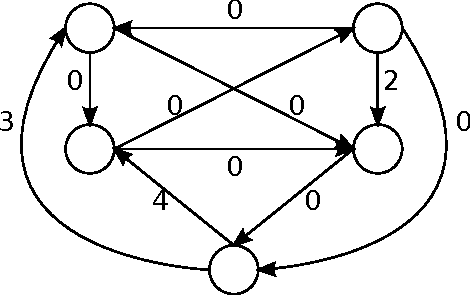
\includegraphics[width=\textwidth/2]{graphics/fig1.pdf}
\caption{A $b$-flow for graph 1 a found in the assignment text}
\label{fig:ex1figa}
\end{figure}
There exists no $b$-flow for Figure 1 (b) as vertix $v_4$ has a demand of $-2$, but no outgoing edges, so this demand cannot be met.

\newpage
\section*{Exercise 2}
\subsection*{Question 2.1}
There are thirteen breaking points in Figure 3 of the assignment. Table \ref{tab:innerTurnBreak} show the values of all possible \(z_{fg}\) in Figure 3 of the assignment, where \(f\) is the first column and \(g\) is the first row of the table.
\begin{table}
\centering
$
\left[
\begin{array}{cccccc}
 & a & b & c & d & e \\
a & 0 & 0 & 0 & 0 & 0 \\
b & 2 & 0 & 1 & 1 &  \\
c & 1 & 1 & 0 & 0 &  \\
d & 0 & 1 & 0 & 0 & 2 \\
e & 4 & 0 & 0 & 0 &  \\
\end{array}
\right]
$
\caption{The number of innerturns a row makes with respect to a column at breakingpoint on shared edges of their boundary respective
boundary cycles.}
\label{tab:innerTurnBreak}
\end{table}
Table \ref{tab:valuesOfxvf} show the value of \(x_{vf}\) for each vertex and immediately adjacent faces, where the first column are the vertices and the first row are the faces present in Figure 3.
\begin{table}
\centering
$
\left[
\begin{array}{cccccc}
   & a & b & c & d & e \\
v1 & 0 & 1 & 1 & 0 & 0 \\
v2 & 0 & 0 & 1 & 1 & 0 \\
v3 & 1 & 0 & 1 & 1 & 1 \\
v4 & 0 & 0 & 0 & -1 & 1\\
v5 & 1 & 0 & 0 & 0 & -1\\
v6 & 1 & 1 & 0 & 1 & 1 \\
v7 & 0 & 0 & 0 & 0 & 0 \\
\end{array}
\right]
$
\label{tab:valuesOfxvf}
\caption{Matrix showing all values $x_{vf}$ where $v$ is the vertex and $f$ is the boundary cycle.}
\end{table}
The rectilinear layout of the graph from Figure 2(a) in the assignment text can be seen in Figure \ref{fig:ex21figa}.
\begin{figure}[H]
\centering
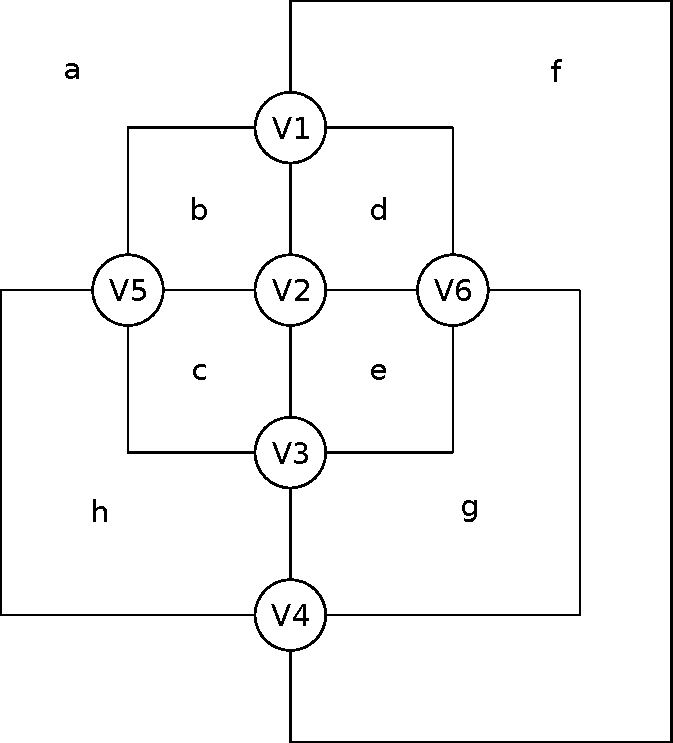
\includegraphics[width=\textwidth / 2]{graphics/fig2.pdf}
\caption{Rectilinear layout of graph Figure 2(a) in the assignment given the planar embedding in Figure 2(b).}
\label{fig:ex21figa}
\end{figure}


\subsection{Question 2.2}
We let $V$ be the set of all vertices. To find the number of outer turns subtracted from the inner turns, we calculate $\sum_{v\in V} x_{vf}$ as outer turns will count as $-1$ and inner turns will count as $1$. It is $0$ otherwise which means the vertex is either on a straight line or is not on the boundary cycle $f$.

We let $G$ be the set of all boundary cycles except the boundary cycle we are looking at. To account for the breakpoints, inner turns in $f$ are given by $\sum_{g\in G} z_{fg}$. The outer turns in $f$ can be found by $\sum_{g\in G} z_{gf}$. Notice that if the faces $f$ and $g$ are not adjacent to each other, the value of $z_{gf}$ is treated as $0$. We can then state the constraints as

\begin{align*}
\sum_{v\in V} x_{vf}+\sum_{g\in G} z_{fg}-\sum_{g\in G} z_{gf} &=
\begin{cases}
-4 & \text{if $f$ is the external face} \\
4  & \text{otherwise}
\end{cases}
\end{align*}

Using Table \ref{tab:innerTurnBreak} and Table \ref{tab:valuesOfxvf} we can verify that our linear constrains hold. To verify the linear constraint holds for face \textbf{a} we sum over the first column in Table \ref{tab:valuesOfxvf} to obtain that \(x_{v\textbf{a}}=3\), we sum over the first column in Table \ref{tab:innerTurnBreak} to obtain \(z_{\textbf{a}g} = 0\) and finally sum over the first row in Table \ref{tab:innerTurnBreak} \(z_{g\textbf{a}} = 7\). Plugging the values into our linear constraint we obtain the expected \(-4\) for face \textbf{a}. Following the same procedure with face \textbf{e}, ie. summing over the fifth column in Table \ref{tab:valuesOfxvf}, and the fifth column and row in Table \ref{tab:valuesOfxvf}, we obtain \(x_{v\textbf{e}}=2\), \(z_{\textbf{b}g} = 4\) and \(z_{g\textbf{b}} = 2\). Plugging these values into our linear constraint we obtain the expected value of 4 for face \textbf{e}.

\subsection*{Question 2.3}
If we allow that vertices can have a higher degree than $4$, we can not construct a rectilinear layout as it by definition only consists of horizontal and vertical lines. \\
To show :
\begin{align*}
\sum_{f} x_{vf} &=
\begin{cases}
0 & \text{if $v$ has degree 2} \\
2 & \text{if $v$ has degree 3} \\
4 & \text{if $v$ has degree 4}
\end{cases}
\end{align*}
We observe that the sum of all angles between edges incident to \(v\) must be \(360^\circ\) and that these can only be horizontal or vertical with respect to each other. From this it follows that two edges incident to the same \(v\) can either have smallest angle \(180^\circ\) or \(90^\circ\).

When the vertex has degree $2$, there is either two straight angles or there is one right angle and one that is $270^{\circ}$. Both will sum to $0$ as two straight angles will be $0+0$ while the other case is $1-1$.

When the vertex has degree $3$, the only composition of angles is two right angles and one straight angle. This will sum to $2$.

When the vertex has degree $4$, the only possible solution is that each $x_{vf}$ is $1$, thus summing to $4$, as there are only right angles.
Thus we have shown that the only possible values of \(\sum_{f} x_{vf}\) are the described cases.

\subsection*{Question 2.4}
The objection function is to minimize the number of break points. This can achieved by minimizing all $z_{fg}$ for all combinations of $f$ and $g$. Together with the constraints found in (2.2) and (2.3) and the final constraint in the assignment text, we can formulate the linear program as
\begin{equation}
\begin{array}{rrll}
&\text{Min:} & \sum_{f}\sum_{g\backslash\{f\}} z_{fg} &\\
\hline
&\text{s.t.} & \sum_{v\in V} x_{vf}+\sum_{g\in G} z_{fg}-\sum_{g\in G} z_{gf} &=
\begin{cases}
-4 & \text{if $f$ is the external face} \\
4  & \text{otherwise}
\end{cases} \\
& & \multicolumn{1}{r}{\sum_{f} x_{vf}} &=
\begin{cases}
0 & \text{if $v$ has degree 2} \\
2 & \text{if $v$ has degree 3} \\
4 & \text{if $v$ has degree 4}
\end{cases} \\
& &\multicolumn{1}{r}{z_{fg}} & \geq 0, \mbox{ for all faces $f$ and $g$}
\end{array}
\end{equation}
This linear program includes all three constraints and an objective function.

\section*{Exercise 3}
We are given an instance $I_0$ of GMCFP, a directed graph $G=(V,E)$ with values of $l_e$, $u_e$, $b_v$ and $c_e$.

\subsection*{Question 3.1}
Consider an instance $I_0$, where the lower and upper capacities are $-\infty$ and $\infty$ respectively.
\begin{figure}[H]
\centering
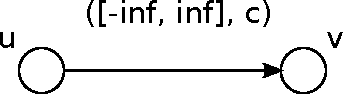
\includegraphics[width=\textwidth / 2]{graphics/fig3.pdf}
\label{fig:ex30fig}
\end{figure}
The instance \(I_1\) is a modification to instance \(I_0\) where we finitely bind the capacity either from above or below.
We do this by splitting the edge \((u,v) \in E(I_0)\) with cost \(c \in \mathbb{R}\) and capacity in the range $[-\infty ,\infty]$ into two more edges and a vertex:
\begin{figure}[H]
\centering
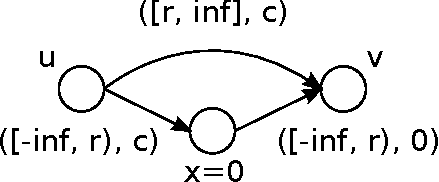
\includegraphics[width=\textwidth / 2]{graphics/fig4.pdf}
\label{fig:ex31fig}
\end{figure}
where $r\in \mathbb{R}$. The demand for the added vertex $x$ is $0$. 
if the minimal flow still produces the same minimum cost as it is applied to both edge $(u,v)$ and $(u,x)$ (but not to the edge $(x,v)$ as it would produce double cost).

\subsection*{Question 3.2}
To assure all the lower capacities $l_e$ for all edges $e$ are finite, we make all edges with capacities $[-\infty, r)$ 
with \(r \in \mathbb{R}\) and cost function $c_e$ into edges going the opposite direction with capacities $[-r, \infty]$ and cost function $-c_e$. For example, if we apply this step to the instance $I_1$ from (3.1), we get
\begin{figure}[H]
\centering
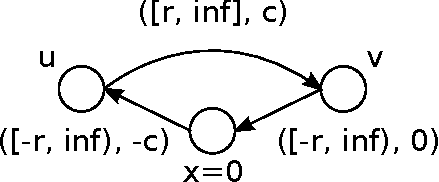
\includegraphics[width=\textwidth / 2]{graphics/fig5.pdf}
\label{fig:ex32fig}
\end{figure}
These are equivalent as sending $x_e$ units over an edge with cost $c_e$ as negative flows can be seen as positive flows in the other direction.

\subsection*{Question 3.3}
Now we want to bind all edges from below with $0$. To achieve this, we look at all edges on the form:
\begin{figure}[H]
\centering
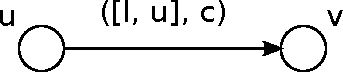
\includegraphics[width=\textwidth / 2]{graphics/fig6.pdf}
\label{fig:ex33figa}
\end{figure}
where $l$ is the lower capacity and $u$ is the upper capacity. We can make an equivalent instance by adding a vertex with demand $-l$ and another edge. This produces two edges. The edge $(y,v)$ is changed to have capacities $[0,u]$ with cost $c_e$. The other edge, $(u,y)$, gets capacities $[0,u-l]$ with cost $0$ (note the upper limit could also be $\infty$, but it can never be larger than $u-l$). This is illustrated here:
\begin{figure}[H]
\centering
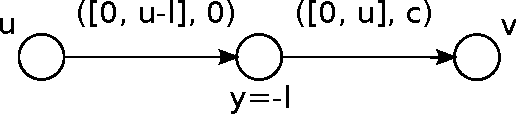
\includegraphics[width=\textwidth / 2]{graphics/fig7.pdf}
\label{fig:ex33figb}
\end{figure}

\subsection*{Question 3.4}
For the instance $I_0$, we have $\abs{E}$ edges. For each edge in instance $I_0$, we can at most create 4 new vertices, $1$ from $I_0$ to $I_1$ and $3$ from $I_2$ to $I_3$, and $5$ edges, $2$ from $I_0$ to $I_1$ and $3$ from $I_2$ to $I_3$. This gives us a total of $6\abs{E}$ edges and $4\abs{E}+\abs{V}$ vertices for instance \(I_3\) which is $\mathcal{O}(\abs{V}+\abs{E})$.
\end{document}